
\subsubsection{Spectrum Info}
Displays information about loaded spectra, both from files (which ones, write out) and detectors memory.
\begin{figure}[H]
    \centering
    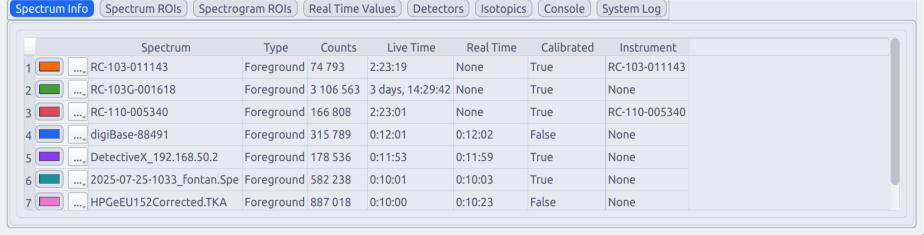
\includegraphics[width = .9\linewidth]{images/interface/spectrum_tab.jpg}
    \caption{Spectrum Info Tab. For imported spectra with other formats than \texttt{XML} or \texttt{N42} file extensions are kept in the name.}
    \label{fig:spectrum_info}
\end{figure}

\begin{table}[H]
    \centering
    \caption{Description of the columns in the Spectrum Info tab}
    \label{tab:spectrum_info_table}
    \begin{tabular}{p{.3\textwidth}p{.64\textwidth}}
    \toprule
    \textbf{Column} & \textbf{Description} \\ \midrule
        Column 0 & Color button allowing for changing the color of the displayed. Options button marked with '...', see \autoref{tab:spectrum_info_options_menu}. \\
        Spectrum & The name of the spectrum or connected detector. A spectrum retrieved from a detector is automatically given the same name as the detector, this can not be changed unless the spectrum is saved or exported. \\
        Type & \textit{Foreground} or \textit{Background}, these share the same name in the 'Spectrum'-column for the same spectrum. This division exists because a spectrum can contain both foreground and background that have different measurement times and total counts. \\
        Live Time & The live time (h:min:s) of the measurement, accounting for dead time. \\
        Real Time & The real time (h:min:s) of the measurement. \\
        Calibrated & \textit{True} or \textit{False}, if an energy calibration is detected and applied. \\
        Instrument & Which instrument is assigned to the spectrum, see section \ref{sec:definitions} \\
    \bottomrule
    \end{tabular}
\end{table}

\begin{table}[H]
    \centering
    \caption{Description of the options menu opened by the button marked '...' on each row. The type 'Background's are limited to only the 'Remove' option.}
    \label{tab:spectrum_info_options_menu}
    \begin{tabular}{p{.3\textwidth}p{.64\textwidth}}
    \toprule
    \textbf{Field} & \textbf{Description} \\ \midrule
        Save & Save the spectrum to the Data Library. \\
        Export & Export the spectrum to a standalone file in the following formats: \texttt{XML}, \texttt{CSV}, \texttt{xlsx}. \\
        Hide/Show & Toggle visibility of the spectrum in the spectrum view. ROIs are not applied to hidden spectra. \\
        Edit & Edit properties of the spectrum, see \autoref{}. \\
        Remove Spectrum & Remove the spectrum and disconnect a detector associated with the spectrum.
    \\ \bottomrule
    \end{tabular}
\end{table}